\section{Introduction}

% --- Slide 1: The Challenge ---
\begin{frame}{Can an Evolutionary Algorithm Play Pac-Man?}

	The goal of this project is to train a neural network to master the classic arcade game, Pac-Man.
	This non-trivial task requires the agent to develop complex strategies for:

	\begin{minipage}{0.55\textwidth}

		\vspace{0.5em}
		
		\begin{itemize}
			\item Efficient maze navigation
			\vspace{0.5em}
			\item Dynamic evasion of multiple, intelligent opponents (ghosts)
			\vspace{0.5em}
			\item Strategic use of resources (power-ups)
			\vspace{0.5em}
			\item Long-term planning to clear the entire level
		\end{itemize}
		
		\vspace{1em}
	\end{minipage}%
	\hfill
	\begin{minipage}{0.45\textwidth}
		\centering

		\vspace{-0.5em}

		\begin{figure}
			\centering
			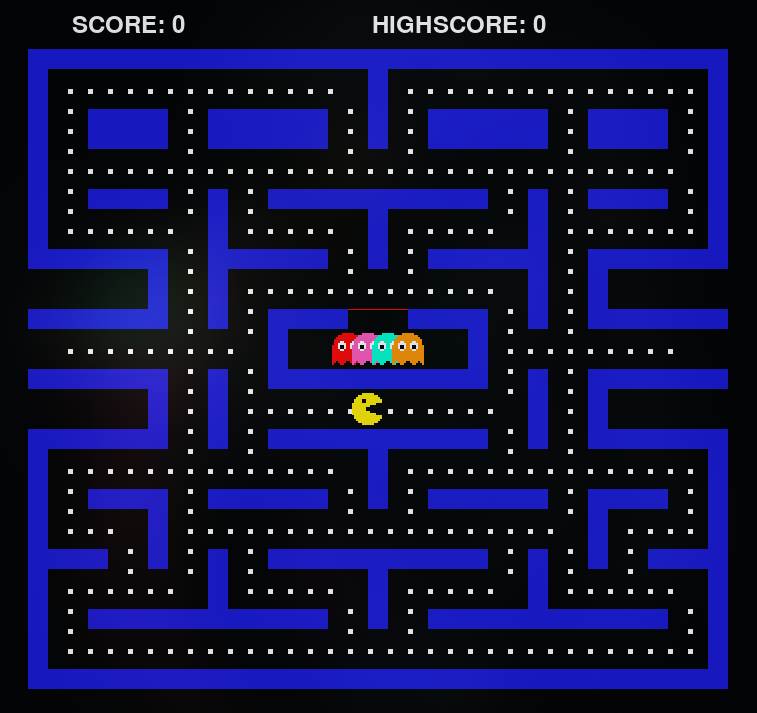
\includegraphics[width=0.82\linewidth]{assets/maze.png} % Usa una tua immagine di Pac-Man

			\caption{\centering \small Pac-Man environment}
		\end{figure}

		\vspace{-1em}
	\end{minipage}

	Instead of traditional programming, It's possible to use an evolutionary approach to \textbf{discover} these strategies automatically.
\end{frame}

\begin{frame}{NEAT - NeuroEvolution of Augmenting Topologies}
		We use \textbf{NEAT} \cite{stanley2002evolving}, a powerful algorithm that evolves both the \textbf{weights} and the \textbf{structure (topology)} of neural networks.

		Key features of NEAT:
		\begin{itemize}
			\item \textbf{Complexification:} Starts with simple networks and gradually adds nodes and connections.
			\item \textbf{Innovation Numbers:} Tracks the historical origin of genes to solve the "competing conventions problem" during crossover.
			\item \textbf{Speciation:} Groups similar networks to protect new innovations until they're ready to compete.
		\end{itemize}

		\vspace{-0.5em}
		
		\begin{figure}
			\centering
			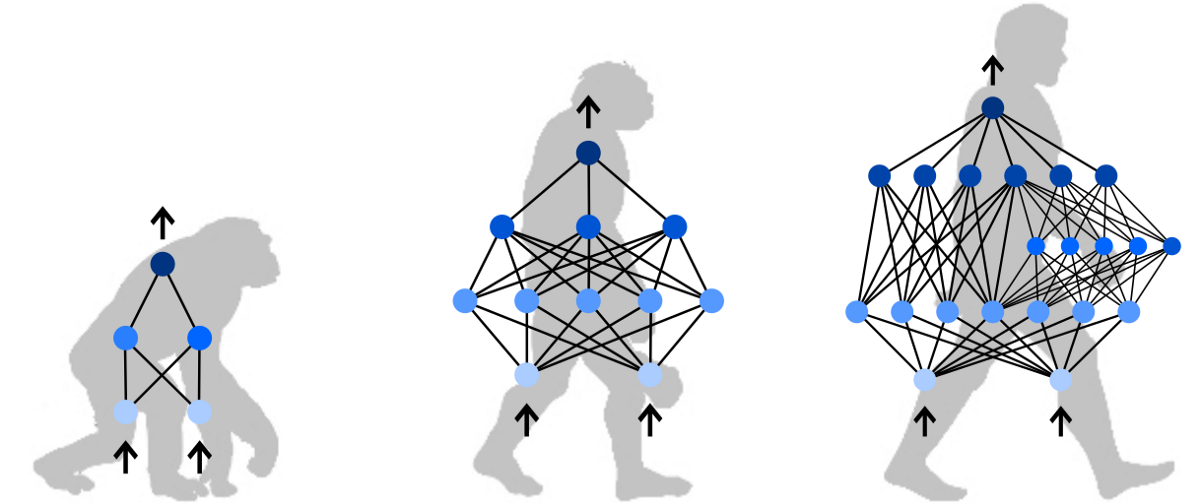
\includegraphics[width=0.55\linewidth]{assets/neat-evolution.png}
			\caption{NEAT increases network complexity over time \cite{shrestha2025reinforced}.}
		\end{figure}

\end{frame}



\begin{frame}{Choosing a Game Environment}
	
	For training NEAT agents, I chose the \textit{PyPacman} environment~\cite{pypacman}.

	\vspace{0.5em}

	\textbf{Advantages:}
	\begin{itemize}
		\item Lightweight and easy to understand
		\item Fully open-source and modifiable
		\item Minimal dependencies
	\end{itemize}
	This enables \bfit{rapid simulation of thousands of games per generation}.

	\vspace{1em}

	\textbf{Limitations:}
	\begin{itemize}
		\item Contained several bugs and inconsistencies
		\item Not optimized for large-scale, automated runs
	\end{itemize}

	\vspace{1em}

	The repository provided a solid foundation, but required several changes to meet the needs of this project:
	\begin{itemize}
		\item Fixed bugs, optimized performances
		\item Added a \bfit{Gym-like interface} for agent-environment interaction
	\end{itemize}

\end{frame}

\begin{frame}{Project Architecture}
	The project integrates the NEAT algorithm with a Pac-Man environment.

	\vspace{1.5em}

	\begin{columns}[T]
		\begin{column}{0.5\textwidth}
			\textbf{Pac-Man Game Engine}
			\begin{itemize}
				\item Adapted from \textit{PyPacman} \cite{pypacman}.
				\vspace{0.5em}
				\item Refactored game state management.
				\vspace{0.5em}
				\item Core logic encapsulated in a Gym-like environment.
			\end{itemize}
		\end{column}
		\begin{column}{0.5\textwidth}
			\textbf{NEAT Framework}
			\begin{itemize}
				\item \texttt{trainer.py}: Manages the evolutionary loop, population, and checkpoints.
				\vspace{0.5em}
				\item \textbf{Parallel Evaluation:} Evaluates genomes simultaneously to speed up training.
			\end{itemize}
		\end{column}
	\end{columns}
	

	\vspace{1em}
	
	\begin{figure}
	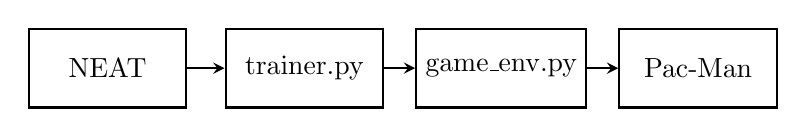
\begin{tikzpicture}[node distance=2.5cm, >=stealth, thick]
		\node (neat) [draw, rectangle, minimum width=2cm, minimum height=1cm] {NEAT};
		\node (trainer) [draw, rectangle, minimum width=2cm, minimum height=1cm, right of=neat] {trainer.py};
		\node (game_env) [draw, rectangle, minimum width=2cm, minimum height=1cm, right of=trainer] {game\_env.py};
		\node (pacman) [draw, rectangle, minimum width=2cm, minimum height=1cm, right of=game_env] {Pac-Man};
		\draw[->] (neat) -- (trainer);
		\draw[->] (trainer) -- (game_env);
		\draw[->] (game_env) -- (pacman);
	\end{tikzpicture}
	\caption{High-level interaction between NEAT and the game environment.}
	\end{figure}
\end{frame}
